%!TEX root = ./00_thesis.tex
%!GEDIT texmaster = ./00_thesis.tex

\chapter{Motivation}

Prozessorientierung ist eine nicht mehr wegzudenkende Maxime in der Gestaltung von Unternehmen. Sie ist ein wesentlicher Bestandteil der Forschung in der Be- triebswirtschaftslehre und der Wirtschaftsinformatik.

Process orientiation is a precept in business organization. It is an essential part of research in business adminstration as well as \acrfull{IS}. To make use of it, models as the language of \acrshort{IS} take an important part. In particular, the reference models support businesses in these reorganization projects. They guide the user and help to incorporate best and common practices so that there is solid foundation to customize the model for the businesse's originalities.  

Outsourcing customer service to external providers is a common practice throughout many industries. Dialling a contact number for a service request often ends up with talking to a service agent anywhere around the world. Several companies have specialized to provide professional customer support using various contact channels. Providing customer relationship management (CRM) as service requires the careful and cost-efficient deployment of contact centres. Such centres are often staffed with hundreds of agents that must be hired and trained before customer contact.
For years, special focus has been put on the voice channel (Loudhouse, 2013). Meanwhile digital trends have affected many areas of life, which implies new challenges in customer relationship management. A recent study revealed that 78.7\% of call centre operations managers point out that their current systems fail to meet future needs, as they are telephone-centric and costs for an architecture overhaul are too high (Dimension Data, 2015). Nowadays consumers can use a plethora of devices and software applications to interact with organizations (Köffer, Ortbach and Niehaves, 2014). As a result, the number of used channels to reach organizations increases. More specifically, analysts have seen a move from the traditional voice channel to digital channels, such as chat or social media. For instance, private instant messengers offer faster and less complicated ways to interact with the company. Digital channels in contact centres now take 42\% of overall interactions and are said to overtake voice by the end of 2016 (Dimension Data, 2016). To this end, multichannel CRM has become a “must-have” for customer service management providers (Agnischock et al., 2015).
In this context, the term omnichannel CRM is increasingly dragging intention. Omnichannel CRM can be distinguished from multichannel CRM by not only providing multiple channels for customer interaction but also through seamless integrations of various channels and their underlying data (Verhoef, Kannan and Inman, 2015), which is a difficult task in CRM. At this point in time, omnichannel CRM is often not realized. However, customers more and more expect that they are able to switch between interaction channels without the loss of information. Contact centre interactions will often require the customer to repeat information again, although he or she has earlier written an email or a chat message to the same company.
Omnichannel CRM also comes with important benefits for organizations. Integrated data throughout various channels allows getting a better understanding of the customer’s profile and wishes through analytical support. Still, 40\% of contact centres have no data analysis tool in place despite of being named the top factor to shape the industry in the next five years (Dimension Data, 2015). 
To this end, organizations can better target marketing campaigns or increase the quality of service provision. To realize this, organizations that use outsourcing need close relations to outsourcing providers, since the integration of channels affects various information systems both at the organization but also at the outsourcing provider. More specifically, CRM business processes need to be harmonized since they often span organizational boundaries.


 

Outsourcing processes have be

	\begin{itemize}
		\item Janina BA
		\item ECIS Paper
		\item Refmod motivation Püster?
		\item Omnichannel 
		\item purpose statement
		\item research question and hyptoheses
	\end{itemize}

	\begin{itemize}
		\item Crewsell: State problem, 
		\item review studies that have addressed the problem,
		\item  indicate definciencies in studies, 
		\item advance significance, 
		\item state purpose statement
	\end{itemize}
%%%%%%%%%%
\chapter{Methodology}
%%%%%%%%%%
	\section{Overview}
	%%%%%%%%%%		
		\begin{itemize}
			\item Creswell Preliminary Cosiderations:
			\item 1Selection of Research Approach
			\item epistemology (sarker2013)
			\item 2Litreview
			\item 3UseofTheory ?
			\item 4Writing Strategy?
			\item Figure for my approach
		\end{itemize}
	
	
	\begin{tikzpicture}
	[node distance=.6cm,
	start chain=going below,]
	\node[punktchain, join] (investeringer)      {Investeringsteori};
	\node[punktchain, join] (perfekt) {Det perfekte kapitalmarked};
	\node[punktchain, join, ] (emperi) {Emperi};
	\node (asym) [punktchain ]  {Asymmetrisk information};
	\begin{scope}[start branch=venstre,
	%We need to redefine the join-style to have the -> turn out right
	every join/.style={->, thick, shorten <=1pt}, ]
	\node[punktchain, on chain=going left, join=by {<-}]
	(risiko) {Risiko og gamble};
	\end{scope}
	\begin{scope}[start branch=hoejre,]
	\node (finans) [punktchain, on chain=going right] {Det finansielle system};
	\end{scope}
	\node[punktchain, join,] (disk) {Det imperfekte finansielle marked};
	\node[punktchain, join,] (makro) {Investeringsmssige konsekvenser};
		\node[punktchain, draw=pink] (aux1) { };
	\node[punktchain, below right=0.6cm and -1.975cm of makro] (konk) {Konklusion};
	\node[punktchain,  left = of konk,] (konk2) {Konklusi2on};
		\node[punktchain, below= of aux1 ] (m1) {m1};
	% Now that we have finished the main figure let us add some "after-drawings"
	%% First, let us connect (finans) with (disk). We want it to have
	%% square corners.
	\draw[|-,-|,->, thick,] (finans.south) |-+(0,-1em)-| (disk.north);
	\draw[|-,-|,->, thick,] (emperi.south) |-+(0,-1em)-| (risiko.north);
	\draw[|-,-|,->, thick,] (emperi.south) |-+(0,-1em)-| (asym.north);

\draw[|-,-|,->, thick,] (makro.south) |-+(0,-0.7em)-| (konk.north);
\draw[|-,-|,->, thick,] (makro.south) |-+(0,-0.7em)-| (konk2.north);

\draw[|-,-|,->, thick,] (konk.south) |-+(0,-0.7em)-| (m1.north);
\draw[|-,-|,->, thick,] (konk2.south) |-+(0,-0.7em)-| (m1.north);

	% Now, let us add some braches. 

	\draw[tuborg, decoration={brace}] let \p1=(perfekt.north), \p2=(emperi.south) in
	($(2.5, \y1)$) -- ($(2.5, \y2)$) node[tubnode] {Problemfelt};
	\end{tikzpicture}
		\begin{itemize}
			\item Designing research Creswell
			\item eventuell grafik aus ecis paper? 
		\end{itemize}
	%%%%%%%%%%
	\section{Literature Review}
	%%%%%%%%%%
	%kann ich erst zum Schluss schreiben
		\begin{itemize}
			\item Where, How, For what
			\item später: was wurde konkret durchsucht und wo? 
		\end{itemize}
	%%%%%%%%%%
	\section{Empirical Research}
	%%%%%%%%%%
Drawing on core principles of qualitative research (Creswell, 2014), this research uses diverse data collection methods. 
%interviews
%data, --> ECIS paper draft. 
% analysis of papers?
	
		\begin{itemize}
			\item Qualitative Methods
			\item Interviews, how many, how long, with whom, sample
			
		\end{itemize}
	%%%%%%%%%%
	\section{Design Science}
		\begin{itemize}
			\item Hefner, Peffers. Draw line complete the view of used research methods.
			\item item
		\end{itemize}
%%%%%%%%%%
\chapter{Research Background}
	%%%%%%%%%%
	DEFINITIONS DEFINITIONS DEFINITIONS
	\section{Domain}
	%%%%%%%%%%
		%%%%%%%%%%
		\subsection{Business Process Outsourcing}
		%%%%%%%%%%
		As put by Thomas Friedman, "The world is flat". Globalization facilitates  combinations value-creating activities in economical networks like never before. The key driver of it is information technology, which sets the base for the connectedness we take for granted today. Its implications on markets and businesses are described in the following section. 
		
		\subsubsection{Theory of the Firm}
		In theory, a firm exists because of transaction and production costs efficiencies. They are organizational innovations to reduce costs involved in market transacting. A transaction here means the transfer of a good or service across a technologically separable interface \cite{williamson1981economics, williamson1971vertical}, like the boundaries between firms. If the transaction costs across markets become larger than the costs of managing the firm, firms will substitute market transactions through internal execution. IT has drastically reduced these transaction costs.
		The theory of production cost efficiency states that production by multiple individuals is the characteristic of a firm \cite{alchian1972production} and it will exist as long as the output is sufficiently larger than the output under independent production, so that the costs organization of individuals are justified. When scale economies of management and production are high, the production cost efficiencies will therefore also increase. As an asset's productivity increases with specialization, this in return explains why firms specialize in certain tasks: costs of managing the firm increase with size,  benefits in productivity are reachable through focusing on their core business.
		When a firm makes its core business to parts that others do not choose to, they can provide these as a service on the market place - and decreasing transaction costs make it more and more attractive to make us of these. 
		
		\subsubsection{The value chain}
		Drawing on the concept of the value chain by Porter //todocite, the idea is to model each firm as a set of systems, which add value to a product or service. These chains can be concatenated, as more and more actors are involved on the way to the end consumer. Within each chain for a firm lie different subsystems, which contribute to the created value through the consumption of resources - like money, labor or material. Strategy demands that firms build sustainable competitive advantages to be able to survive in the market. As firms cannot build these in all stages of their value chain \cite{Ramachandran2004}, they choose to focus in certain activities and hence invest less resources in others. 
		
		Combining the previously mentioned theory of the firm and concept of the value chain, organizations may transfer activities to other actors in the market that have specialized on it and can deliver it better and more efficient.  
		
			\subsubsection{Outsourcing}
		The term outsourcing can be derived from \textbf{out}side re\textbf{sourcing} and dates back to 1981. It is characterized by contracting out (part of) a process to another party. However, it does not necessarily mean relocating it to a foreign country (offshoring), which falsely gave the term a negative connotation in Germany in the past \footnote{ "Outsourcing" was chosen the Un-word of the year 1996 \url{http://www.unwortdesjahres.net/index.php?id=33}}. Outsourcing can be distinguished by other types of partnerships through a contract that clearly defines subject and duration of the cooperation. Processes in which IT plays an important role became prime candidates for outsourcing, as transaction costs for information are negligible. More sharply, one can speak of \acrfull{ITES} that can be outsourced using the power of IT \citep[\p{49}]{Ramachandran2004}. 
				
		\acrshort{BPO} is a special form of outsourcing. In contrast to traditional outsourcing, BPO is defined as the transfer of complete processes to another business, which are called vendors or providers. BPO refers to the delegation of one or more information technology enabled processes to an external service provider. 
		
		\subsubsection{Process orientation}
		
	The concept of processes is a central part of this thesis. As it turns out, there a conflicts in the wording between the business process management and outsourcing domain. A process is defined a self-contained time-logical sequence of activities that work on a business relevant object. \citep[\p{6}]{becker2012pm}. A business process is a special process that is directed by the business objectives of a company and by the business environment \citep[\p{6}]{becker2012pm}. This definition needs to be carefully separated from the notion within Business Process Outsourcing, which only stresses the outsourcing of complete processes and does not necessarily limit its applicability to business processes as defined here. The author notes that BPO is a common term and it is therefore mandatory to use it to correctly describe the domain. However, for the act of process modeling, the distinction between processes and business processes is necessary. An example for this conflict is that outsourcing the payroll management process would be considered BPO, while the very nature of the process is clearly not directed by the business objectives of the company. 
	
	Porters value chain differentiates into primary and supporting activities. The former are directly contributing to the created product or service and therefore have impact on the economic outcome of the company. Logistics, Operations or Service are parts of these primary activities. Supporting activities on the other hand do not have a direct relatedness to the product or service, but are necessary to perform primary activities. Human resource management or IT can be named here. This distinction between primary and support activities may be flowing and leaves room for interpretation and is additionally dependent on the business domain and company itself. The concept of the two activities is borrowed and applied to processes that shall be distinguished in core and support processes. 
	 

		
		\subsubsection{A framework for BPO participants}
	There are at least two parties involved in an outsourcing setting. The business that is outsourcing a process is called \textit{client} in this setting, while the business that is servicing the outsourced process is called \textit{provider}. This thesis focuses on building a model for the provider and takes its perspective. Due to this view, it is also referred to as the focal company. With respect to the outsourced process, there additionally may be \textit{customers} involved. These can be other businesses or private consumers. CRM services are such an example, as customers of the client contact the provider to solve a service request for instance. \ref{fig:bpochain} visualizes the described B2B2B/C chain as an analogy on B2B and B2C as existing shorthands for business-to-business and business-to-consumer. The following describes the case with an involved customer group. The chain underlines the two critical intersections of the focal company with the other markets. It is important to stress these as markets instead of two business partners or the alike: An outsourcing provider has multiple clients (each having customers that may be part of the BPO) and hence their business can be modeled as multiple chains with different client and customers. However, each chain is centered by the focal company. Consequently these form a market that the provider interacts with.
	
			\begin{figure}[caption={BPO B2B2B/C Chain}, label={fig:bpochain}]
		{	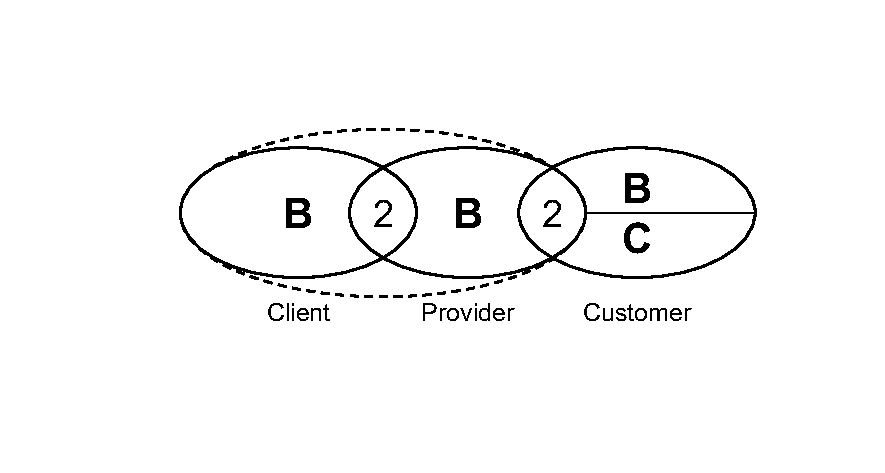
\includegraphics[width=.8\textwidth]{figures/bpochain.pdf}}
	\end{figure}

			
		\begin{itemize}
			\item motivation optional 
			\item history optional
			\item process orientation  ok
			\item DEF
			\item common processes that are outsourced - zahlen
			\item schewe 3: venn diagramm prozesoptimierung - bpo - outsourcing
			
			\item IT as an enabler
			\item offshore, nearshore, inshore - nur nennen und auf interessante Aspekte für case eingehen
			\item Model ? Matrix ? 
			\item Outsourcing Chain muss hier sein 
		\end{itemize}
	
		\subsubsection{Parent Company}
		%% irgendwie wiederkehrende Struktur bei Parent Company und Provider...
		Motivation for outsourcing of services is based on sound economic principles. 
		\begin{itemize}
			\item reasons: focus on core competencies
			\item fields // processes no29 for India, Deloitte Outsourcing Paper
			\item challenges
			\item 
		\end{itemize}
		\subsubsection{Outsourcing Provider}
		
		\begin{itemize}
			\item dienstleistungsstruktur  : schewe
			\item no29: intro to firms, transaction costs so on
			\item no29: capabilities of Providers
		\end{itemize}
		%%%%%%%%%%
		\subsection{Customer Relationship Management}
		%%%%%%%%%%
		Customer acquisition costs are the price a company pays to gain a new customer. The existing customer base does not require this spending. In addition, a strong relationship to customers offers more sales, \ie more revenue generated through the individual. Consequently, firms strive to build relationships with their customers to make them loyal consumers of their goods and services. The rise of information technology enabled \acrfull{CRM}. which builds on relationship marketing and adds the orientation towards information in practice. In academics both terms are often used interchangeably \cite{ryals2001customer}.  Having its origin in the mid 90s with the IT community, there is no agreed definition of	\acrshort{CRM} to this day. \cite{paynefrow2005} compiled different standpoints and propose three views, that will be described in the following. As the name suggests, the building and sustaining of relationships to customers is always a defining characteristic of \acrshort{CRM}, but the importance of the technological component is varying. 
		
		Narrowly and tactically defined, \acrshort{CRM} refers to a technology solution and its implementation. With an increased scope, \acrshort{CRM} can be seen as the implementation of an integrated series of customer-oriented technology solutions. Widely and strategically defined, \acrshort{CRM} can be seen as a holistic approach to managing customer relationships to maximize customer value, corporate profitability, and thus, shareholder value \cite{payne2004role}. This value is realized through the developed of a relationship, that is profitable and preferably long-term. 
	
		For this thesis, a customer is defined as an individual or business that has entered the process of buying a good or service from another business. Hence, the customer has a relation to the latter, that is of interest in CRM. This relationship can be strengthened by a plethora of marketing instruments that businesses use to bind the customer. These are initiated from the businesses and directed towards the customer. The reverse way, \ie, a customer reaching to the company is also possible.  
				%process view 
		\subsubsection{Digital Channels}
		\subsubsection{Non-Digital Channels}
		
		42: stems from mid 90s, IT community. can be seen as informatin-enabled relationship marketing. 3 perspectives: narroly and tactical: implementation of a specific technology solution project. mid: implementation of a series of integrated customer-oriented tech solutions. broadly: crm is a holsitc approach to manage customer relationships to create shareholder value. channel split is old eCommerce does not make sense anymore.
		process view of payne frow helps, as it is not limited by organizational aspects. 
				\begin{itemize}
			\item CSM or CM or CRM?
			\item Value Chain - GoM PDF -- könnte man auch bei RefMod / Ordnungsrahmen machen. 			
			\item Importance for businesses
			\item characteristics, developments 
			\item payne/frow
		\end{itemize}
	
	\subsubsection{Multi-Channel CRM}
		%janina
	\subsubsection{Omni-Channel CRM}
	    %janina
	 
		%%%%%%%%%%
		\subsection{Customer Relationship Management Business Process Outsourcing Providers}
		%%%%%%%%%%
		\begin{itemize}
			\item ECIS Paper...
			\item Strategy, Capabilities from voleti concretized. 
			\item one face to the customer
			\item B2B2X
			\item virtual company
		\end{itemize}
	%%%%%%%%%%
	\section{Reference Modeling}
	%%%%%%%%%%
		%%%%%%%%%%
		\subsection{Concept}
		
		\subsubsection{The Model as a construct}
		
		
		
		\begin{itemize}
			\item kurz geschichte
			\item eigenes subheading für modellbegriff?
			\item 
		\end{itemize}
		Reference Models can be seen as theory of information systems \cite{Schutte1998}. A model itself is defined as an "immaterial representation of an original for the purposes of a subject" \citep[\p{1}]{Becker2012Gom}. Based on the work of \cite{Stachowiak1973}, three characteristics of models are identified: mapping, reduction and pragmatism.  Mapping describes the representation of natural or artificial originals, which can be models themselves. Reduction underlines the omission of certain elements of the original in a model. Pragmatism means that the selection of parts of the original is dependent on the intent of the model. Based on this notion, models of information systems (or information models in short) are explicit models that have information systems as subject matter. Information modeling, the act of creating these, is a complex task, which is why reference models provide a useful means to reduce the effort \cite{Becker2007}. \cite{thomas2006refmod} compiles various definitions for reference models. 
		
		%mehr auf definitionen eingehen
		For this thesis, a reference model is defined as an information model with content that is reused in the construction of other information models \cite{Becker2004}.
		
		Companies show growing individuality in their processes with increasing granularity. A reference model therefore needs to be as precise as possible, while maintaining the claim of being reusable. Approaches to find \textit{the} reference model that encompasses various domains stand in contrast to practical use, as the application of a very general reference model gets more and more effortful due to its abstract and theoretical nature \citep[\p{79}]{Schutte1998}. Striking a balance between these trade-offs is known as the reference modeling dilemma. The literature shows, that a defined application domain is a necessary ground for fruitful reference modeling.
		
		  %delfmann: Variantenmanagement
		  
			%grafik aus refmod - enzyklopädie vom brocke
		A model is always created by one or multiple subjects. This group shall be called designers and is in the context of reference modeling responsible for the reference model itself. The designer implements requirements from the reference model user. The idea behind is \textit{design for reuse} in contrast to application model side, where \textit{design with reuse} is the prevailing concept. There, one can identify an application model constructor and application model user. Akin to the reference model designer, the constructor takes requirements from the application model user. The difference is that he uses the reference model as the basis for adaption. By doing this, the application can represent characteristics of the application environment, while still being conformable to the reference model. As time proceeds, the reference and application model evolve and change states. As the name suggests, reference model can be used in multiple application model construction processes as they are typically tailored to a specific domain,\enquote{\eg}, retail, manufacturing or supply chain management.
		
		%languages noch ausführlicher?
		
		
		%types: data, organizational
		Information models can focus on different aspects of information systems. Drawing from the  \acrfull{ARIS}, one could take five different perspectives on \acrshort{IS}: organizational,functional, data, output and process. These perspectives can be motivated by \textit{pragmatism} as a model characteristic. The complexity of reality is reduced in a model through abstraction from insignificant parts for the purpose. From an organizational perspective responsibilities may be of highest importance, while they do not take this role in the data perspective. There, on the other hand, other aspects are essential like data entities and their relationships. 
		
		
		% der Process
		\subsubsection{Process orientation}
		% process def ist aber schon bei bpo 
		 The process view is located in the center of \acrshort{ARIS}, integrating information from the organizational, functional, output and data context. 
				
	
		
		\subsubsection{Selected Reference Models}
		
		The purpose of this section is to briefly present two different reference models that are used in practice: The \acrfull{SCOR} Model and the Retail-H. Both show a layer structure to manage complexity and both encompass a process reference model. 
		
		\acrshort{SCOR} allows modelling of supply chains. It is a process reference model with three detail levels. It was developed in 1996 and is now maintained by the Association for Operations Management \cite{APICS2015}. On the highest level, typically called regulatory framework, \acrshort{SCOR}  is based on six distinct management processes: Plan, Source, Make, Deliver, Return and Enable. While the regulatory framework assists in defining scope, the second configures the type of supply chain (Make-to-Order, Build-to-Order, Engineer-to-Order). On the thirds level these are decomposed into generic process steps (e.g., issue product). Even more detailed processes are considered company specific and therefore no part of the model. Furthermore, performance metrics are also defined on each level. 

		\begin{figure}[caption={SCOR Model}, label={fig:scor}]
		{	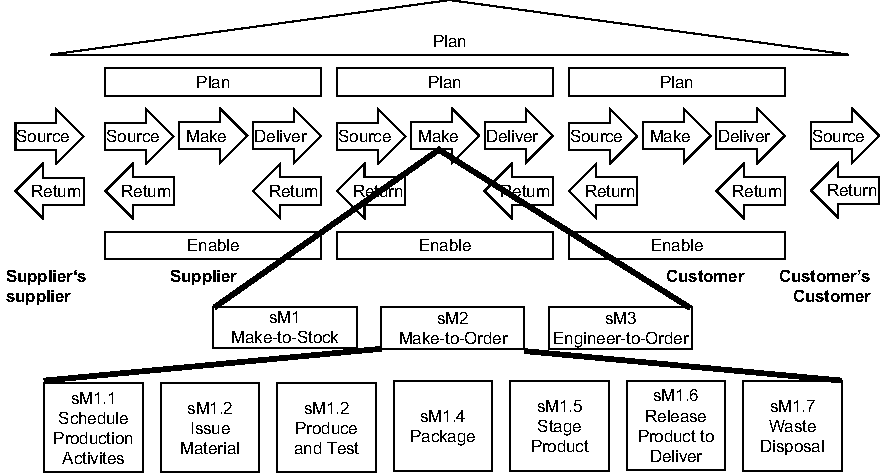
\includegraphics[width=.8\textwidth]{figures/scor.pdf}}
		\end{figure}
	

		In the domain of retail, the Retail-H is a reference model that includes process, function and data models. Developed by \cite{Becker2004a}, it has been adapted to suit special segments of the domain (for instance eCommerce, Central Clearance, Central Settlement). 
		It is structured along four levels of detail: the regulatory framework, main processes, detail processes and process building blocks. The core of the regulatory framework is made up of three parts that form the H (a connection to the German word for retail: “Handel”). While the left part of the H describes the supply side, the right covers the distribution side. Both are connected through logistics. All of these core processes are business processes, the roof and foundation consist of support processes thereby making use of the framework reference design as proposed in \cite{Meise2001}. 
		Each segment on the regulatory framework is a main process, that has several main process steps and each of these is a detail process. The detail process steps are process building blocks and show the highest level of detail. 
		\begin{figure}[caption={Retail-H}, label={fig:retailh}]
			{	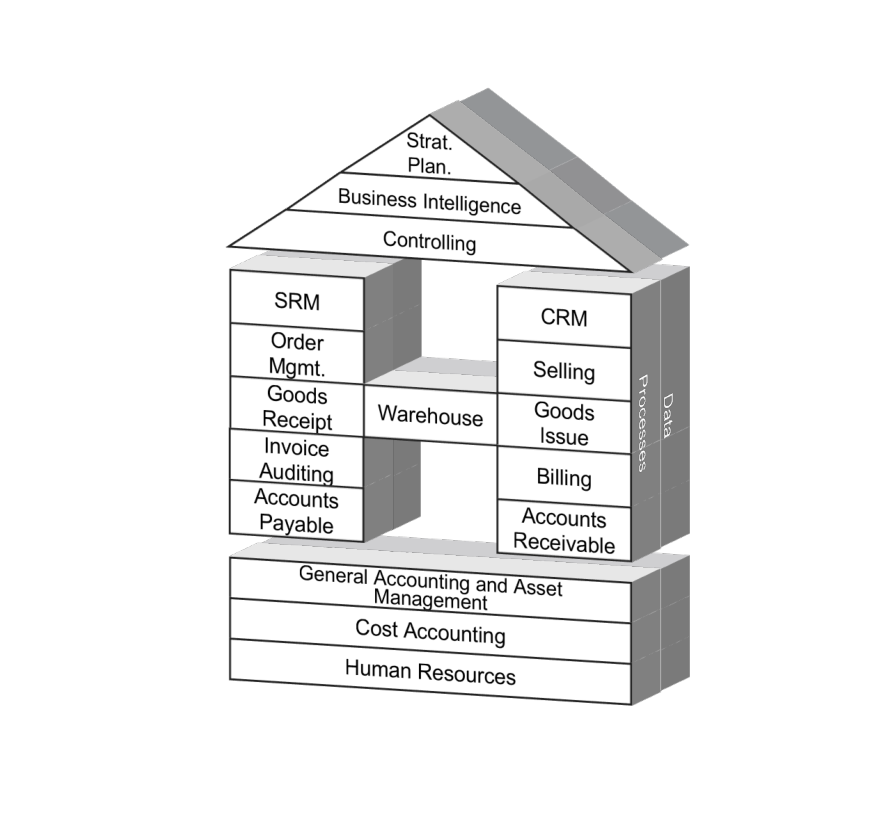
\includegraphics[width=.6\textwidth]{figures/retailh.pdf}}
		\end{figure}
		
		%%%%%%%%%%
	
	
	
		%%%%%%%%%%
		\subsection{Construction}
		vielleicht hier die model levels erklären? - Nein, das ist mein Beitrag. Muss in RefModConstruction 
		%%%%%%%%%%
		%%%%%%%%%%
		\subsection{Benefits}
		%%%%%%%%%%
		\begin{itemize}
			\item  ECIS paper part!
			\item TODO: Fragen ob man hier schon auf bpo crm aspekte eingeht... eigentlich schon. was bringen die allgemeinen denn. 
			\item auch vom Brocke checken 
		\end{itemize}
		%%%%%%%%%%
		\subsection{icebricks as a Process Modeling Language}
		
	 Fundamental for a language is the ability to communicate through use of it. As this thesis focuses on process modeling, the  Basic concepts of a modeling language are tied to its purpose. Traditional modeling languages like EPCs, Petri-Nets or BPMN are very similar. Being a syntactical language, they offer large degrees of freedom in usage. What might look like an advantage at first sight, turns out to be disadvantageous. As process management approaches have increased number and variety of model designers and users enormously, more and more non-experts get in contact with process models and thus creating models of less quality. The definition of modeling conventions becomes necessary to help the modeler to conform to certain standards. A way to confront this challenge are the \acrfull{GOM}, which are an analogy to the \acrfull{GAAP}. However, conforming to these guidelines will lead to an increase resource requirements in these undertakings. The concept of semantic process modeling languages avoid this by enforcing additional rules that models have to follow. icebricks is one example that realizes this concept. In addition to syntactical correctness, \ie conforming to the language's meta model, other aspects are also considered which would otherwise be taken care of by combining \acrshort{GOM} and syntactical languages. Because the additional check for guideline compliance is unnecessary in semantic languages, they are more efficient. In the following the \acrshort{GOM} are described and it is argued why icebricks conforms to the aspects. 
	 
	 \subsubsection{Correctness}
	 
	 \subsubsection{Relevance}
	 
	 \subsubsection{Economic efficiency}
	 
	 \subsubsection{Clarity}
	 
	 \subsubsection{Comparability}
	 	
	 \subsubsection{Systematic Design}
	 To 
		%%%%%%%%%%
		\begin{itemize}
			\item Icebricks paper von design science conf
			\item Retail Tabelle mit Features aufdröseln 
			\item Warum so Referenzmodellierung machen? Noch nich auf case gehen, das ist background
		\end{itemize}
	
	\begin{itemize}
		\item Correctness
			\subitem simple processes against high complexity
		\item Relevance - GoB: completeness does not make sense
			\subitem simple processes against high complexity
		\item Economic efficiency
		\subitem no longer correction of defects a posteriori. 
		\item clarity
			\subitem glossary against naming conflicts
			\subitem 4 layers against missing orientation structure
			\subitem simple processes against high complexity
		\item comparability 
			\subitem glossary against naming conflicts
			\subitem 4 layers against missing orientation structure
			\subitem simple processes against high complexity
		\item systematic design 
			\subitem  4 layers against missing orientation structure
			\subitem simple processes against high complexity
	\end{itemize}
\chapter{Case}
%%%%%%%%%%
\begin{itemize}
	\item Arvato talk in general
	\item numbers
	\item history
	\item DSR applied here
	\item vom Brocke grafik begründet mein Vorgehen + DSR
\end{itemize}
%%%%%%%%%%
\section{DSR Application for Arvato}
%%%%%%%%%%
\begin{itemize}
	\item wie wende ich DSR hier an?
	\item warum wende ich DSR hier an?
	
\end{itemize}
%%%%%%%%%%
\section{Problem Identification}
%%%%%%%%%%
\begin{itemize}
	\item Kraume interview, process interviews
	\item historisch gewachsen
	\item verschiedener sprech
	
\end{itemize}
%%%%%%%%%%
\section{Solution Objective and Stakeholders}
%%%%%%%%%%
\begin{itemize}
	\item Kraume interview
	\item Stakeholders
	\subitem Sales
	\subitem PSD / IT
	\subitem Ops
\end{itemize}
%%%%%%%%%%
\section{Limitiations}
%%%%%%%%%%
\begin{itemize}
	\item only core processes specified, as also done in retail-h
	\item core processes partly on lowest level
	\item process refmod, not data
	\item specified later
\end{itemize}
%%%%%%%%%%

\chapter{Reference Model Construction}
%%%%%%%%%%
\begin{itemize}
	\item Approach from Case advanced to the model itself
	
\end{itemize}
\subsubsection{A proposed Architecture for Reference Models in BPO}
	%%%%%%%%%%
	\section{Process Framework}
	%%%%%%%%%%
	\begin{itemize}
		\item meise 2001
	\end{itemize}
	%%%%%%%%%%
	\section{Internal Services}
	%%%%%%%%%%
	%%%%%%%%%%
	\subsection{...}
	%%%%%%%%%%
	%%%%%%%%%%
	\section{Client Services}
	%%%%%%%%%%
	%%%%%%%%%%
	\subsection{...}
	%%%%%%%%%%
	%%%%%%%%%%
	\section{Customer Services}
	%%%%%%%%%%
	%%%%%%%%%%
	\subsection{...}
	%%%%%%%%%%
	%%%%%%%%%%
\chapter{Evaluation}
%%%%%%%%%%
	%%%%%%%%%%
	\begin{itemize}
		\item 
	\end{itemize}
	%%%%%%%%%%
	\section{Internal Services}
	%%%%%%%%%%
	%%%%%%%%%%
	\section{Client Services}
	%%%%%%%%%%
	%%%%%%%%%%
	\section{Customer Services}
	%%%%%%%%%%
	%%%%%%%%%%
\chapter{Conclusion}






\chapter{Sample}
This \LaTeX \- template has been developed as an alternative to the well-known Microsoft Word \enquote{Becker-Vorlage}. \path{00_thesis.tex} is the master file.

It is build by  Jan Betzing and Dominik Lekse and draws from the DBIS template by Till Haselmann and Florian Stahl, as well as from the IS template by Stephan Dlugosz.

This document is work-in-progress and provides instructions on how to use the template. It does not give advices on scientific writing.

Please feel free to contribute to this template. Members of the WWU M\"{u}nster can request access to the template by contacting the author at \href{mailto:jan.betzing@ercis.uni-muenster.de}{jan.betzing@ercis.uni-muenster.de}. Afterwards you will be able to clone the template from \path{https://wiwi-gitlab.uni-muenster.de/lsis/isthesis.git}, and create push-requests with their new features.

\paragraph{TODO}
\begin{itemize}
	\item Configuration switch for having \textbackslash chapter\{\} begin on a new page
	\item Replace \texttt{kvoptions} with \texttt{pgfkeys}
\end{itemize}
\section{Elements}
This chapter gives examples on what you can do with this template. It's just a brief overview. Please consult the common sources on how to write sicentific documents and documents with \LaTeX.

\section{Structure}
This template provides three structural levels that appear in the table of contents, \viz, \texttt{\textbackslash chapter}, \texttt{\textbackslash section}, and \texttt{\textbackslash subsection}. Chapters will always start on a new page. Additionally, you can use \texttt{\textbackslash subsubsection} and \texttt{\textbackslash paragraph} as non-hierarchical means to structure your thesis.


\subsection{Lists}
You can use the default \LaTeX \- functions for writing lists, \viz, \texttt{\textbackslash enumerate} for numbered lists and \texttt{\textbackslash itemize} for bullet point lists. Again, the \texttt{\textbackslash subsubsection} and \texttt{\textbackslash paragraph} can be used as structural elements, \eg, when listing definitions of terms.

\subsection{Footnotes}
Footnotes are contiguously numbered throughout the whole document. Use the \texttt{\textbackslash footnote\{text\}} command.  They appear on the page their reference is on \footnote{This is an exemplary footnote.}. Footnotes have to be placed without whitespace behind the word and within the sentence boundaries, \ie, before the period.

\subsection{ToDo-Notes}
You can use ToDo notes using the \texttt{\textbackslash todo\{text\}}  command. Please make sure to remove any ToDo notes before handing in your thesis! \todo[inline]{ToDo: Remove me before publishing}

\section{Formatting Text}
\LaTeX \- provides \texttt{\textbackslash textit\{text\}} for \textit{italics}, \texttt{\textbackslash textbf\{text\}} for \textbf{bold face}, \texttt{\textbackslash texttt\{text\}} for \texttt{typewriter}, \texttt{\textbackslash textsc\{text\}} for \textsc{small caps}, \texttt{\textbackslash underline\{text\}} for \underline{underline}. Additionally, the template provides  \texttt{\textbackslash texthl\{text\}} for \texthl{highlighted text}. Please remove any highlighted text before handing in your thesis!

Please use the \texttt{\textbackslash enquote\{text\}} command for \enquote{direct quotes}.

\subsection{Colors}
This template comes with the colors defined in the \glspl{CD} of the \acrshort{ERCIS} and \acrshort{WWU}. \Tab \ref{tab:colors} lists the color names. You can apply them to text by using the  \\ \texttt{\textbackslash textcolor\{color name\}\{text\}} command.
	
\begin{table}[caption={Colors defined by the template}, label=tab:colors]
	\centering
		\begin{tabular}{@{}ll@{}}
			\toprule
			{\bf Color Name} & {\bf Result} \\ \midrule
			ercis-black      & \textcolor{ercis-black}{Exemplary Text and 0123456789}  \\
			ercis-grey      & \textcolor{ercis-grey}{Exemplary Text and 0123456789}  \\
			ercis-red      & \textcolor{ercis-red}{Exemplary Text and 0123456789}  \\
			ercis-lightred      & \textcolor{ercis-lightred}{Exemplary Text and 0123456789}  \\
			ercis-blue      & \textcolor{ercis-blue}{Exemplary Text and 0123456789}  \\
			ercis-darkblue      & \textcolor{ercis-darkblue}{Exemplary Text and 0123456789}  \\
			ercis-cyan    & \textcolor{ercis-cyan}{Exemplary Text and 0123456789}  \\
			ercis-orange      & \textcolor{ercis-orange}{Exemplary Text and 0123456789}  \\
			ercis-green      & \textcolor{ercis-green}{Exemplary Text and 0123456789}  \\ \midrule
			wwu-black      & \textcolor{wwu-black}{Exemplary Text and 0123456789}  \\
			wwu-green      & \textcolor{wwu-green}{Exemplary Text and 0123456789}  \\
			wwu-lightgreen      & \textcolor{wwu-lightgreen}{Exemplary Text and 0123456789}  \\
			wwu-blue     & \textcolor{wwu-blue}{Exemplary Text and 0123456789}  \\
			wwu-lightblue      & \textcolor{wwu-lightblue}{Exemplary Text and 0123456789}  \\ \bottomrule
		\end{tabular}
\end{table}


\section{Figures}

The \texttt{figure} environment is wrapped around images. These images should either be included as PDF-file via \texttt{\textbackslash includegraphics}, or created via \textit{TikZ/PGF}. For included images, make sure to use high-resolution images, preferably vector images.

Figures float, \ie, they do not necessarily appear at exact the same position you have defined them. Make sure to set a  \textit{caption} and an optional \textit{label} as figure parameters. 

\begin{figure}[caption={Relationship of students and theses}, label={fig:img01}]
	{	
\includegraphics[width=.6\textwidth]{figures/figure01.pdf}}
\end{figure}

\subsection{Subfigures}
Sometimes it might be handy to contrast figures, \ie, by placing them next to each other. The template uses the \textit{subcaption} package to provide subfigures. The following example contains two figures, where each subfigure has its own \texttt{\textbackslash label} and \texttt{\textbackslash caption}. Additionally, the whole figure has its own \textit{caption} and \textit{label}. That means, you can reference subfigures  \fig \ref{fig:subfig1} and \fig  \ref{fig:subfig}. Only the whole figure will be listed in the table of figures.

Subfigures are not limited to images, but may also include listings or tables. \Fig \ref{fig:subfig} shows a sample database query expressed in \ac{SQL} (\fig \ref{fig:subfig1}) and as query plan in relational algebra  (\fig \ref{fig:subfig2}).
 
\begin{figure}[caption={Exemplary use of subfigures}, label={fig:subfig}]
	
	\begin{subfigure}[b]{.45\textwidth}
		
		\begin{lstlisting}[nolol, language=SQL]
		SELECT b, d FROM 
			EXAMPLE.RELATION1 r,
			EXAMPLE.RELATION2 s,
		WHERE 
			r.a = 'c'
		AND 
			s.e = 2
		AND 
			r.c = s.c; 
		\end{lstlisting}
		\caption{\gls{SQL} select statement}\label{fig:subfig1}
	\end{subfigure}
	\begin{subfigure}[b]{.53\textwidth}
		\centering	
		\begin{tikzpicture}[node distance = 2cm, auto,
		database/.style={
			cylinder,
			cylinder uses custom fill,
			cylinder body fill=gray!30,
			cylinder end fill=gray!20,
			shape border rotate=90,
			aspect=0.25,
			draw
		}]
		\node [] (queue) {$\Pi_{b, d}$};
		\node [below of=queue] (join) {$\Join_{r.c = s.c}$};
		
		\node [below left of=join,xshift=-1cm] (l1) {$\sigma_{r.a = 'c'}$};
		\node [database, below of=l1] (l2) {\texttt{r}};
		
		\node [below right of=join,xshift=1cm] (r1) {$\sigma_{s.e = 2}$};
		\node [database,below of=r1] (r2) {\texttt{s}};
		
		\draw [<-] (queue) -- (join);
		\draw [<-] (join) -- (r1);
		\draw [<-] (r1) -- (r2);
		\draw [<-] (join) -- (l1);
		\draw [<-] (l1) -- (l2);
		\end{tikzpicture}
		\caption{Sample evaluation plan}\label{fig:subfig2}
	\end{subfigure}
\end{figure}
\section{Listings}
You can use listings to typeset source code. This template uses the \textit{listings} package. Wrap code inside the \texttt{lstlisting} environment and set the \textit{language} (e.g., Java, SQL), \textit{caption}, and optional \textit{label} parameters. If the source code highlighting highlights the wrong keywords or misses keywords, use the \textit{deletekeywords} \resp \textit{morekeywords} parameters. Consult the package documentation for further information.

\begin{lstlisting}[float=htp, caption={Euclid's GCD algorithm implemented in Java}, label={lst:euclid}, language=Java, deletekeywords={}, morekeywords={}]
public class Euclid {

	public static int gcd(int p, int q) {
		if (q == 0) return p;
		else return gcd(q, p % q);
	}

}
\end{lstlisting}

\section{Algorithms}
Some users might require specifying algorithms. This template uses the \textit{algorithm}, \textit{algorithmicx}, and \textit{algopseudocode} packages. Consult the respective manuals for further information. Algorithms do not appear in a table at the beginning of the document, \ie, there is no list of algorithms.

\begin{algorithm}[htb]
	\begin{algorithmic}
		\Require nonnegative integer $a$, nonnegative integer $b$
		\Function{Euclid}{$a, b$}
		\If {$b = 0$} \Comment{comment}
		\State{return $a$;}
		\Else 
		\State {return \textsc{Euclid}$(b, a\mod b)$;}
		\EndIf
		\EndFunction
	\end{algorithmic}
	\caption{Euclid's GCD algorithm in pseudocode}
	\label{alg:garbage}
\end{algorithm}

\section{Acronyms and Abbreviations}
This template provides comprehensive support for acronyms and abbreviations. The template uses the \textit{glossaries} package. 
Please do only define abbreviations and symbols that are uncommon. That means, common abbreviations such as \enquote{\eg} or \enquote{\ie} should not be listed. Abbreviations and symbols are sorted automatically by their label. 

\subsection{Common Abbreviations}
Please note that each full stop in a common abbreviation should be followed by a non-breaking space. This template comes with a variety of macros for common abbreviations, that can be used throughout your theses. The macros differ for English and German theses. Please see the tables below.

\begin{table}[caption={Common abbreviation macros for English theses}, label=tab:macros1]
	\centering
	\begin{tabular}{@{}ll@{}}
		\toprule
		{\bf Command} & {\bf Result} \\ \midrule
			\textbackslash apprx      & \apprx \\
			\textbackslash as      & \as \\
			\textbackslash cf      & \cf \\
			\textbackslash eg      & \eg \\
			\textbackslash Eg      & \Eg \\
			\textbackslash esp      & \esp \\
			\textbackslash etal      & \etal \\
			\textbackslash fig      & \fig \\
			\textbackslash Fig     & \Fig \\
			\textbackslash ie      & \ie \\
			\textbackslash Ie      & \Ie \\
			\textbackslash iid      & \iid \\
			\textbackslash p\{4711\}      & \p{4711} \\
			\textbackslash pf\{4711\}      & \pf{4711} \\
			\textbackslash pp\{11$--$47\}      & \pp{11--47} \\
			\textbackslash resp      & \resp \\
			\textbackslash sect     & \sect \\
			\textbackslash tab      & \tab \\
			\textbackslash Tab      & \Tab \\
			\textbackslash viz      & \viz \\
			\textbackslash wrt      & \wrt \\ \bottomrule
	\end{tabular}
\end{table}

\begin{table}[caption={Common abbreviation macros for German theses}, label=tab:macros2]
	\begin{subfigure}[t]{.45\textwidth}
	\centering
	\begin{tabular}{@{}ll@{}}
		\toprule
		{\bf Command} & {\bf Result} \\ \midrule
\textbackslash aaO & \mbox{a.\,a\,O}\xdot \\
\textbackslash Abb & \mbox{Abb.~} \\
\textbackslash bspw & \mbox{bspw}\xdot \\
\textbackslash bzgl & \mbox{bzgl}\xdot \\
\textbackslash bzw & \mbox{bzw}\xdot \\
\textbackslash ca & \mbox{ca}\xdot \\
\textbackslash dgl & \mbox{dgl}\xdot \\
\textbackslash dsgl & \mbox{dsgl}\xdot \\
\textbackslash dh & \mbox{d.\,h}\xdot \\
\textbackslash etc & \mbox{etc}\xdot \\
\textbackslash eV & \mbox{e.\,V}\xdot \\
\textbackslash evtl & \mbox{evtl}\xdot \\
\textbackslash fs & \mbox{f.\,s}\xdot \\
\textbackslash gdw & \mbox{g.\,d.\,w}\xdot \\
\textbackslash ggf & \mbox{ggf}\xdot \\
\textbackslash hc & \mbox{h.\,c}\xdot \\
\textbackslash iAllg & \mbox{i.\,Allg}\xdot \\
\textbackslash iBa & \mbox{i.\,B.\,a}\xdot \\
\textbackslash idR & \mbox{i.\,d.\,R}\xdot \\
\textbackslash ieS & \mbox{i.\,e.\,S}\xdot \\
\textbackslash inkl & \mbox{inkl}\xdot \\
\textbackslash insb & \mbox{insbes}\xdot \\
\textbackslash Prof & \mbox{Prof}\xdot \\
\textbackslash Dr & \mbox{Dr}\xdot \\
\textbackslash PD & \mbox{PD}\xdot \\
\textbackslash Ing & \mbox{Ing}\xdot \\
\textbackslash iV & \mbox{i.\,V}\xdot \\
\textbackslash iW & \mbox{i.\,W}\xdot \\
\textbackslash iwS & \mbox{i.\,w.\,S}\xdot \\
\textbackslash Nr\{123\} & \mbox{Nr.~123} \\
\textbackslash nW & \mbox{n.\,W}\xdot \\
\textbackslash oa & \mbox{o.\,a}\xdot \\
\textbackslash oAe & \mbox{o.\,\"{A}}\xdot \\
			\textbackslash oae & \mbox{o.\,\"{a}}\xdot \\\bottomrule
\end{tabular}
\end{subfigure}
	\begin{subfigure}[position=t]{.45\textwidth}
		\centering
		\begin{tabular}{@{}ll@{}}
			\toprule
			{\bf Command} & {\bf Result} \\ \midrule

			\textbackslash oE & \mbox{o.\,E}\xdot \\
			\textbackslash oEdA & \mbox{o.\,E.\,d.\,A}\xdot \\
			\textbackslash OEdA & \mbox{O.\,E.\,d.\,A}\xdot \\ 
			\textbackslash oV & \mbox{o.\,V}\xdot \\
			\textbackslash OV & \mbox{O.\,V}\xdot \\
			\textbackslash resp & \mbox{resp}\xdot \\
			\textbackslash S\{123\} & \mbox{S.~123} \\
			\textbackslash Sf\{123\} & \mbox{S.~123~f}\xdot \\
			\textbackslash Sff\{123\} & \mbox{S.~123~ff}\xdot \\
			\textbackslash siehe & \mbox{s.\,o}\xdot \\
			\textbackslash sog & \mbox{sog}\xdot \\
			\textbackslash sS\{123\}  & \mbox{s.\,S.~123}\\
			\textbackslash sSf\{123\} &\mbox{s.\,S.~123~f}\xdot \\
			\textbackslash sSff\{123\}& \mbox{s.\,S.~123~ff}\xdot \\
			\textbackslash stu & \mbox{st.\,u}\xdot \\
			\textbackslash su & \mbox{s.\,u}\xdot \\
			\textbackslash Tab & \mbox{Tab.~} \\
			\textbackslash tw & \mbox{t.\,w}\xdot \\
			\textbackslash ua & \mbox{u.\,a}\xdot \\
			\textbackslash etal & \mbox{et\ al}\xdot \\
			\textbackslash uae & \mbox{u.\,\"{a}}\xdot \\
			\textbackslash uAe & \mbox{u.\,\"{A}}\xdot \\
			\textbackslash uiv & \mbox{u.\,i.\,v}\xdot \\
			\textbackslash usw & \mbox{usw}\xdot \\
			\textbackslash uU & \mbox{u.\,U}\xdot \\
			\textbackslash va & \mbox{v.\,a}\xdot \\
			\textbackslash vgl & \mbox{vgl.~} \\
			\textbackslash Vgl & \mbox{Vgl.~} \\
			\textbackslash vs & \mbox{v.\,s}\xdot \\
			\textbackslash zB & \mbox{z.\,B}\xdot \\
			\textbackslash zT & \mbox{z.\,T}\xdot \\
			\textbackslash zz & \mbox{zz}\xdot \\
			\textbackslash zzgl & \mbox{zzgl}\xdot \\
 & \\ \bottomrule
	\end{tabular}
	\end{subfigure}
\end{table}

\subsection{Custom Abbreviations}
Custom abbreviations are defined in the \path{acronyms.tex} file, using the \\
\texttt{\textbackslash newacronym[longplural=\{<long plural>\}, shortplural=\{<short plural>\}]\\ \{<label>\}\{<short>\}\{<long>\}} command. The \textit{longplural} and \textit{shortplural} parameters are optional. The abbreviations are sorted by their labels. The label is furthermore used to reference the abbreviations in your text. You can do so using commands listed in \tab \ref{tab:glossaries}. In most cases, you just use \textbackslash gls\{<label>\}. On the first occurrence, the full version is displayed, \eg, \acrfull{ERCIS}. Afterwards, the short version will be displayed, \eg, \acrshort{ERCIS}.

You pluralize your abbreviation by adding a \texttt{pl} to the \resp command. This will add a small s to the abbreviation, \eg, \acrshortpl{CD}. \Tab \ref{tab:glossaries} shows custom short and long plural versions of the abbreviation \acrshort{kmu}. You might need this \esp for more complex German abbreviations that do not have a \enquote{s} plural form.

\begin{table}[caption={Commands for printing abbreviations}, label=tab:glossaries]
	\centering
	\begin{tabular}{@{}ll@{}}
		\toprule
		{\bf Command} & {\bf Result} \\ \midrule
		\textbackslash gls\{<label>\}     & \textbackslash acrfull on first occurence, \textbackslash acrshort otherwise \\
		\textbackslash glspl\{<label>\}       &  \textbackslash acrfullpl on first occurence, \textbackslash acrshortpl otherwise \\
		\textbackslash acrshort\{<label>\}       & \acrshort{kmu} \\
		\textbackslash acrshortpl\{<label>\}       & \acrshortpl{kmu} \\
		\textbackslash acrlong\{<label>\}       & \acrlong{kmu} \\
		\textbackslash acrlongpl\{<label>\}      & \acrlongpl{kmu} \\
		\textbackslash acrfull\{<label>\}      & \acrfull{kmu} \\
		\textbackslash  acrfullpl\{<label>\}     & \acrfullpl{kmu} \\ \bottomrule
	\end{tabular}
\end{table}

Only referenced abbreviations will be added to the list of abbreviations.

\subsection{Symbols}
If required, you can define symbols in the \path{symbols.tex} file, using the \\ \texttt{\textbackslash addsymboltolist\{<symbol>\}\{<label>\}\{<name>\}} command. The symbols are sorted by their labels. Please note, regardless of using the symbols in the text, all symbols defined in the symbols file will be output to the list of symbols.

\section{Citations and Bibliography}
This template uses {BibTeX} for bibliographies. It comes with the MISQ style that takes care of proper formating and sorting of your references. Of course, you have to maintain a clean \path{.bib} file that caters all necessary attributes. References will appear in the alphabetical order of the surname of the first author. In case of several works by the same author, they are sorted by year.

Citing in the text is done with the \textbackslash citep[<before>][<after>]\{<citekey>\} command. Citations without parenthesis are done with \textbackslash cite\{<citekey>\}. You can reference authors with \textbackslash citeauthor\{<citekey>\}. However, we suggest typesetting authors in \textsc{Small Caps}, \eg, \textsc{\citeauthor{Hammer2015}} is one father of \ac{BPM}.

\paragraph{Exemplary citations}

\begin{itemize}
	\item \gls{BPM} is an integral management paradigm for building and running effective and efficient organizations  \citep{Hammer2015, VomBrocke2014a}.
	\item A holistic approach to \ac{BPM} goes beyond process modeling and workflow management systems \citep[\p{530}]{VomBrocke2014a}.
	\item See \cite{VomBrocke2014a} for a comprehensive review on \ac{BPM} best practices.
	\item \textsc{\citeauthor{Hammer2015}} lists organizational capabilities for \ac{BPM} \citep[\cf][\pf{9}]{Hammer2015}, while \textsc{vom Brocke} \etal give principles of good \ac{BPM} \citep[\cf][\pp{530--546}]{VomBrocke2014a}.
	\item Two authors are automatically divided by an \enquote{and} in English or an \enquote{und} in German, \eg, \citep{Becker2011}.
	\item \enquote{\ac{BPM} can provide a solid set of capabilities essential to master contemporary and future challenges} \citep[\p{534}]{VomBrocke2014a}.
\end{itemize}

\subsection{Misc}
The name and matriculation number of the student will automatically be displayed on the header of every page when the thesis type \textit{seminar} is selected.

\chapter{Compiling the document}
In order to generate a PDF-file from your \TeX-file you have to run the following commands. We assume you have a master file \path{00_thesis.tex} that you want to typeset.

\begin{lstlisting}[float=htp, caption={Commands to compile this document}, label={lst:compiling}, language=bash, morekeywords={pdflatex, bibtex, makeglossaries}]
pdflatex 00_thesis
pdflatex 00_thesis
makeglossaries 00_thesis
bibtex 00_thesis
pdflatex 00_thesis
pdflatex 00_thesis
\end{lstlisting}

Alternatively, you can use your favorite task runner. This thesis comes with a \textit{Grunt} file to kick-start your \LaTeX writing.

When running, Grunt will monitor your thesis and on file changes, the PDF-file is automatically rebuild using the commands from listing \ref{lst:compiling}.
 
Please make sure to have node.js and the \gls{npm} installed. Now you can open a command prompt at the document root and run the commands in listing \ref{lst:grunt}. 

\begin{lstlisting}[float=htp, caption={Installing and running Grunt}, label={lst:grunt}, language=bash]
# Install Grunt via npm (use sudo on Unix-based OS)
npm install -g grunt-cli

# Install Grunt plugins / dependencies
npm install

# Run the Grunt listener 
grunt
\end{lstlisting}

\section{Known Issues}
Under some configurations on Windows machines, the \texttt{makeglossaries} command silently fails, which results in empty lists of accronyms and symbols. Same goes for the implicitly called \texttt{makeindex} command. In this case, you have to install \texttt{Perl}\footnote{https://www.perl.org/get.html} on your machine.